\documentclass[a4paper,12pt]{article}
\usepackage{tikz-feynhand}



\setlength{\feynhandlinesize}{1pt}

\setlength{\feynhandtopsep}{3mm}

\begin{document}

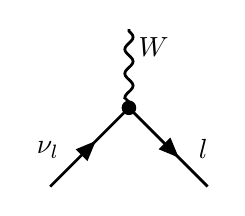
\begin{tikzpicture}[baseline=(o.base)]
    \begin{feynhand}
        \vertex (a) at (-1,-1); \vertex (b) at (1,-1); \vertex (c) at (0,1);
        \vertex [dot] (o) at (0,0) {};
        \propag [fermion] (a) to [edge label=$\nu_l$, near start] (o);
        \propag [anti fermion] (b) to [edge label'=$l$, near start] (o);
        \propag [boson] (c) to [edge label=$W$, near start] (o);
    \end{feynhand}
\end{tikzpicture}

\end{document}